\chapter{Keeping the user in control}\label{chap:control}

\graphicspath{{images/control/}}

\begin{framed}
	\textbf{Key points:}
	
	\begin{itemize}
		\item An experiment was designed to compared \gls{sparc} to another approach in \gls{iml}: \acrfull{irl} using feedback and partial guidance to teach a robot an action policy.
		\item Application domain is a replication of the world used in early studies on \acrshort{irl}.
		\item \gls{sparc} uses full control over the robot's action, implicit rewarding system and evaluation of intentions rather than actions.
		\item \gls{sparc} was combined with \acrlong{rl}.
		\item Results show that \gls{sparc} achieves a better performance, easier and faster than \acrshort{irl}.
	\end{itemize}
\end{framed}

Parts of the work presented in this chapter have been published verbatim in \cite{senft2017supervised} \footnote{Note about technical contribution in this chapter: the author reimplemented every part of the system manually in Qt.}. The final publication is available from Elsevier via \url{https://doi.org/10.1016/j.patrec.2017.03.015}.

\newpage
\section{Motivation}

Previous work in \gls{iml} showed that humans want to teach robots not only with feedback but also by communicating what the robot should do \citep{thomaz2008teachable}. However, in most of the research teaching agents a policy using human guidance, the teacher is given little or no control at all on the agent's actions and has to observe the agent executing an action even when knowing that this action is incorrect. This chapter explores how these \gls{iml} approaches could be pushed further by applying the principles of \gls{sparc} defined in Chapter \ref{chap:sparc}, how it would influence the learning process, the agent performance and the user experience and how these results would compare to other \gls{iml} approaches.

Additionally, the previous study explored how \gls{sparc} could be used with \acrlong{sl}, to replicate a teacher's action policy, but some of the most promising features of \gls{iml} arise when combined with \acrfull{rl}. As such this chapter proposes a way to apply the principles underlying \gls{sparc} to classical feedback based \gls{rl} and evaluates how this human control over the robot's actions impacts the learning. A study involving 40 participants compares \gls{sparc} to another interaction approach offering less control but having been validated in previous studies: \acrfull{irl} \citep{thomaz2008teachable}. The testing environment of \gls{irl} have be reimplemented to stay as close as possible to the online version of the task.

\section{Scope of the study}

\subsection{Interactive Reinforcement Learning}

The \gls{irl} algorithms implements the principles presented in \cite{thomaz2008teachable}: the human teacher can provide positive or negative feedback on the last action executed by the robot and the robot combines this with environmental feedback into a reward which is used to update a Q-table: a table with a Q-values (the expected discounted reward) assigned to every state-action pair and used to select the next action. Three additions to the standard algorithm have been proposed and implemented by Thomaz and Breazeal and are used here as well: guidance, communication by the robot and an undo option \citep{thomaz2008teachable}. Teachers have two way to transmit information to the robot: the reward channel (to give the numerical reward on the last action) and the guidance channel (to direct attention toward parts of the state and restrict exploration).

The guidance emerged from the results of a pilot study where participants assigned rewards to objects to indicate that the robot should do something with these objects. With the guidance, teachers can direct the attention of the robot toward certain item in the environment to indicate the robot that it should interact with them. This guidance behaviour offer partial control over the robot's actions and restricts the next action the robot is executing, but it cannot be used to set explicitly the robot behaviour. 

The robot also communicates its uncertainty by directing its gaze toward different items in the environment with equally high probability of being used next. The aim of this communication of uncertainty is to provide transparency about the robot's internal state, for example indicating when a guidance should be provided. 

Finally, after a negative reward, the robot tries to cancel the effect of the previous action (if possible), resulting in a undo behaviour. As shown in the original paper, these three additions improve the performance on the task.

\subsection{SPARC}

\gls{sparc} uses a single type of input similar to the guidance present in \gls{irl} but without using the reward channel. However with \gls{sparc}, the guidance channel controls directly the actions of the robot. The robot communicates every of its intentions (i.e the action it plans to execute next) to its teacher by looking to a part of the environment and the teacher can either not intervene, letting the robot execute the suggested action or step in and force the robot to execute an alternative action. This combination of suggestions and corrections gives the teacher full control over the actions executed by the robot. This also makes the rewards redundant: rather than requiring the human to explicitly provide rewards, a positive reward is directly assigned to each action executed by the robot as it has been either forced or passively approved by the teacher.

\subsection{Differences of approaches}

Unlike \gls{irl}, \gls{sparc} offers full control over the actions executed by the robot. \gls{sparc} changes the learning paradigm from learning from the human evaluation of actions' effects to learning from the human's expectation of these actions' effects and human's preferences. An expert in the task domain evaluates the appropriateness of actions before their execution and can guide the robot to act as they see fit. This implies that the robot does rely on observing negative effects of an action to learn that this action should be avoided, but rather what the best action is for each state. Even in a non-deterministic environment such as human-robot interactions, some actions can be expected to have a negative consequence and the human teacher can stop the robot from ever executing these actions, preventing the robot from causing harm to itself or its social or physical environment. 

Another noticeable difference is the way in which the robot communicates with the user: in \gls{irl}, the robot communicates its uncertainty about an action and with \gls{sparc} its intention to execute an action. It should also be noted that the quantity of information provided by the user to the robot is similar for both \gls{irl} and \gls{sparc}: in \gls{sparc} the user can offer the whole action space as commands to the robot, which removes the need for explicit rewards. While in \gls{irl}, the teacher can guide the robot toward a subset of the action space but has to manually provide feedbacks to evaluate the robot's decisions.

\subsection{Hypotheses}

Three hypotheses have been tested in the study:
\begin{enumerate}
	\item [H1] \textit{Effectiveness and efficiency with non-experts.} Compared to \gls{irl}, \gls{sparc} leads to higher performance, whilst being faster, requiring fewer inputs and less mental effort from the teacher and minimising the number of errors during the teaching phase when used by non-experts.
	\item [H2] \textit{Safety with experts.} \gls{sparc} can be used by experts to teach an action policy safely, quickly and efficiently, unlike other \gls{iml} methods lacking control.
	\item [H3] \textit{Control.} Teachers prefer a method in which they can have more control over the robot's actions.
\end{enumerate}
\section{Methodology}

The task used in this study is the same as \cite{thomaz2008teachable}: Sophie's kitchen, a simulated environment on a computer where a virtual robot has to learn how to bake a cake in a kitchen. As the source code was not available, the task was reimplemented to stay as close as possible to the description in the paper and the online version of the task\footnote{\url{http://www.cc.gatech.edu/~athomaz/sophie/WebsiteDeployment/}}.

The scenario is the following: a robot, Sophie, is in a kitchen with three different locations (shelf, table and oven) and five objects (flour, tray, eggs, spoon and bowl) as shown in Figure \ref{fig:control_initial}. Sophie has to learn how to bake a cake and the participant has to guide the robot through a sequence of steps while giving enough feedback so the robot learns a correct series of actions. As presented in Figure \ref{fig:control_states}, there are six crucial steps to achieve a successful result:

\begin{enumerate}
	\item Put the bowl on the table (Figure \ref{fig:control_bowl}).
	\item Add one ingredient to the bowl (flour or eggs).
	\item Add the second ingredient (Figure \ref{fig:control_ingredients}).
	\item Mix the ingredients with the spoon to obtain batter (Figure \ref{fig:control_batter}).
	\item Pour the batter in the tray (Figure \ref{fig:control_tray}).
	\item Put the tray in the oven (Figure \ref{fig:control_goal}).
\end{enumerate}

The environment is a deterministic \acrlong{mdp}, defined by a state, a set of actions (move left, move right, pick up, drop and use), a deterministic transition function and environmental reward function (+1 for success and -1 for failure and -0.04 for every other step to penalise long sequences). Different action policies can lead to success, but many actions end in a failure state, for example putting the spoon in the oven results in a failure. As argued by Thomaz and Breazeal, this environment provides a good setup to evaluate teaching methods to a robot due to the large number of possible states (more than 10,000), the presence of success and failure states and the sparse nature of the environmental reward function which increases the need for a teacher to aid the learning. More details on the environment are available in the original paper.

\subsection{Task} \label{ssec:control_task}
\begin{figure}[ht]
	\centering
	\begin{subfigure}[b]{0.3\textwidth}
		\centering
		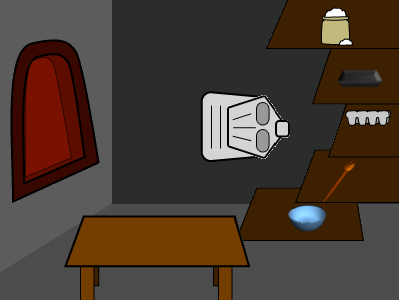
\includegraphics[width=\textwidth]{step0.png}
		\caption{Initial state}
		\label{fig:control_initial}
	\end{subfigure}
	\centering
	\begin{subfigure}[b]{0.3\textwidth}
		\centering
		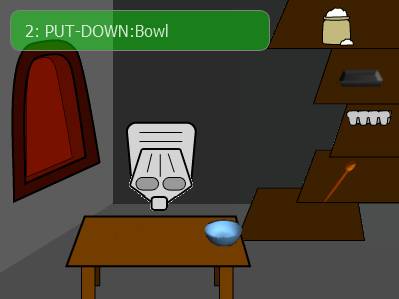
\includegraphics[width=\textwidth]{step1.png}
		\caption{Step 1}
		\label{fig:control_bowl}
	\end{subfigure}
	\centering
	\begin{subfigure}[b]{0.3\textwidth}
		\centering
		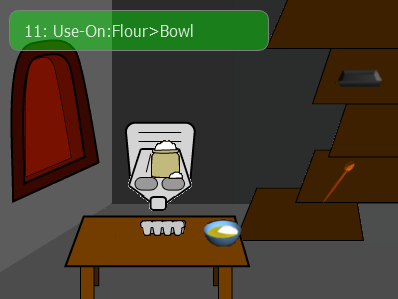
\includegraphics[width=\textwidth]{step3.png}
		\caption{Step 3}
		\label{fig:control_ingredients}
	\end{subfigure}
	
	
	\centering
	\begin{subfigure}[b]{0.3\textwidth}
		\centering
		
\includegraphics[width=\textwidth]{step4.png}
		\caption{Step 4}
		\label{fig:control_batter}
	\end{subfigure}
	\centering
	\begin{subfigure}[b]{0.3\textwidth}
		\centering
		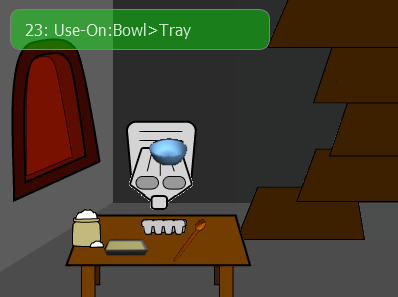
\includegraphics[width=\textwidth]{step5.png}
		\caption{Step 5}
		\label{fig:control_tray}
	\end{subfigure}
	\centering
	\begin{subfigure}[b]{0.3\textwidth}
		\centering
		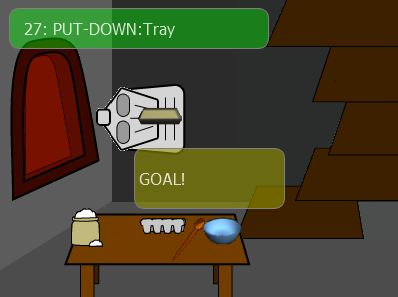
\includegraphics[width=\textwidth]{step6.png}
		\caption{Step 6}
		\label{fig:control_goal}
	\end{subfigure}
	
	\caption{Presentation of different steps in the environment. \ref{fig:control_initial} initial state, \ref{fig:control_bowl} step 1: bowl on the table, \ref{fig:control_ingredients} step 3: both ingredients in the bowl, \ref{fig:control_batter} step 4: ingredients mixed to obtain batter, \ref{fig:control_tray} step 5: batter poured in the tray and \ref{fig:control_goal} step 6 (success): tray with batter put in the oven. (Step 2: one ingredient in the bowl has been omitted for clarity)}
	\label{fig:control_states}
\end{figure}

\subsection{Implementation}

Two conditions are compared for this study: \gls{irl} and \gls{sparc}. The underlying learning is strictly identical for both conditions, only the way to interact with it (inputs to and from the algorithm) and how to provide rewards changes: with \gls{irl} teachers have to explicitly provide rewards, while they are implicit with \gls{sparc}. 

The learning algorithm (see Algorithms \ref{algo:control_sparc} and \ref{algo:control_irl}) is a variation on Q-learning, without reward propagating\footnote{In Q learning the update function is $Q(s_{t},a_{t}) \leftarrow Q(s_{t},a_{t}) + \alpha (r_{t+1}+\gamma (\underset{a}{max} Q(s_{t+1},a))-Q(s_{t},a_{t}))$}. This guarantees that any learning by the robot is due to the teaching by the human, and as such provides a lower bound for the robot's performance. By using Q-learning, the performance of the robot would be higher.

\begin{minipage}[t]{0.5\textwidth}
	\vspace{0pt}  
	\begin{algorithm}[H]
		\caption{Algorithm used for SPARC}
		\label{algo:control_sparc}
		 \While{learning}{
		 	$a$ = action with the highest $Q[s,a]$
		 	
		 	look at object or location used with $a$
		 	
		 	\While{waiting for correction (2 seconds)}{
		 		\eIf{received command}{
		 			$a$ = received command
		 			
		 			reward, $r = 0.5$
		 		}{
		 		reward, $r = 0.25$
		 	}
		 }
		 execute $a$, and transition to $s'$
		 $r = r + r_{environment}$
		 
		 Learn: $Q(s_{t},a_{t}) \leftarrow Q(s_{t},a_{t}) + \alpha (r_{t+1}+\gamma (\underset{a}{max} Q(s_{t},a))-Q(s_{t},a_{t}))$
		}
	\end{algorithm}
\end{minipage}%
\begin{minipage}[t]{0.5\textwidth}
	\vspace{0pt}
	\begin{algorithm}[H]
		\caption{Algorithm used for IRL
			\vspace{0.2pt}}
		\label{algo:control_irl}
		\While{learning}{
			$a$ = action with the highest $Q[s,a]$
			
			indicate confusion if multiple $a$ with similar high $Q[s,a]$
			
			\While{waiting for guidance and reward on last action (2 seconds)}{
				\If{received command}{
					Try: $a$ = received command
				}
				\If{received reward $r'$}{
					$r = r + r'$				
				}
		}
		
		Learn: $Q(s_{t},a_{t}) \leftarrow Q(s_{t},a_{t}) + \alpha (r_{t+1}+\gamma (\underset{a}{max} Q(s_{t},a))-Q(s_{t},a_{t}))$
		execute $a$, and transition to $s'$
		$r = r_{environment}$
		
		\vspace{5.5pt}
	}
	\end{algorithm}
\end{minipage}

As shown in the algorithms, another minor difference between the conditions is that with \gls{sparc}, the algorithm learns just after executing an action (and only with positive rewards), while \gls{irl} learns on the last action before executing the next one based on the human evaluation of the last action.

\subsubsection{Interactive Reinforcement Learning}

We have implemented \gls{irl} following the principles presented in \cite{thomaz2008teachable}. The user can use the left click to display a slider providing rewards. The guidance is implemented by right-clicking on objects: it directs the robot's attention to the object if facing it (a click on objects in different locations has no effect). Following the guidance, the robot will execute the candidate action involving the object. The action space is not entirely covered by this guidance mechanism: for example, it does not cover moving from a location to another. This guidance if used correctly, limits the exploration for the current step to the part of the environment evaluated as more interesting by the user without preventing the robot to explore in further steps. The robot communicates its uncertainty by looking at multiple objects having similarly high probability of being used. 

Some modifications were required to the original study due to the lack of implementation details in the original paper, one of them being the use of a purely greedy action selection instead of using softmax, due to the absence of parameters descriptions. The reliance on human rewards and guidance limits the importance of autonomous exploration, and thus, the greediness of the algorithm should assist the learning by preventing the robot to explore outside of the guided policy. Additionally, as the environment is deterministic and the algorithm is greedy, the concept of convergence is altered: once a trajectory has Q-Values high enough or a correct gradient of Q-Values on all state-action pairs, it will be reinforced automatically. But the teacher can manually force the robot to converge or diverge depending of their behaviours.

\subsubsection{SPARC}

\gls{sparc} uses the gaze of the robot toward objects or locations to indicate which action the robot is suggesting to the teacher. Similarly to the guidance in \gls{irl}, the teacher can use the right click of the mouse on objects to have the robot execute the action associated to this object in the current state and this has been extended to also cover locations. With \gls{sparc}, the command covers all the action space: at every time step, the teacher can specify, if desired, the next action executed by the robot. If an action is not corrected, a positive reward of 0.25 is automatically received (as it has the implicit approval from the teacher) and if the teacher selects another action, a reward of 0.5 is given to the correcting action (the corrected action is not rewarded). That way, actions actively selected are more reinforced and participants can still have give higher rewards when using \gls{irl}. This system allows for the use of reinforcement learning with implicit reward assignation, aiming to simplify the teaching interaction.


\subsection{Interaction protocol}

Participants are divided into two groups and interact first either with \gls{irl} or \gls{sparc} as shown in Figure \ref{fig:control_design}. Before interacting, participants complete a demographic questionnaire and receive an information sheet explaining the task (describing the environment and how to bake the cake) and one explaining the system they are interacting with. Then they interact for three sessions with the assigned system. Each session is composed of a teaching phase and a testing phase. The teaching phase is composed of as many teaching episodes as the participant desires, a teaching episode ends when a success or failure state has been reached which returns the environment to the initial state. In the same way as in the initial experiment by Thomaz and Breazeal, participants can decide to terminate the teaching phase whenever they desire by clicking on a button labelled `Sophie is ready', however the session also stops after 25 minutes to impose an upper time limit to the study. After the end of a teaching phase, the robot runs a testing phase where the participant's inputs are disabled and which stops as soon as an ending state is reached or the participants decide to stop it (for example if the robot is stuck in a loop). This testing phase is used to evaluate the performance of the participants for this session. The interaction with a system consists of three repeated independent sessions with their own independent teaching and testing phases to observe how the interactions evolve as participants are getting used to the system.

After participants completed their three sessions with the first system, they are asked to interact for three more sessions with the other system. This way, every participant interacts three times with each system (\gls{irl} and \gls{sparc}) and the order of interaction is balanced. Additionally, participants have to complete post-interaction questionnaires distributed after the interaction with the first system and the second one and a final post-experiment questionnaire at the end of the experiment. All information sheets and questionnaires can be found online \footnote{\url{https://emmanuel-senft.github.io/experiment2.html}}.

\begin{figure}[t!]
	\centering
	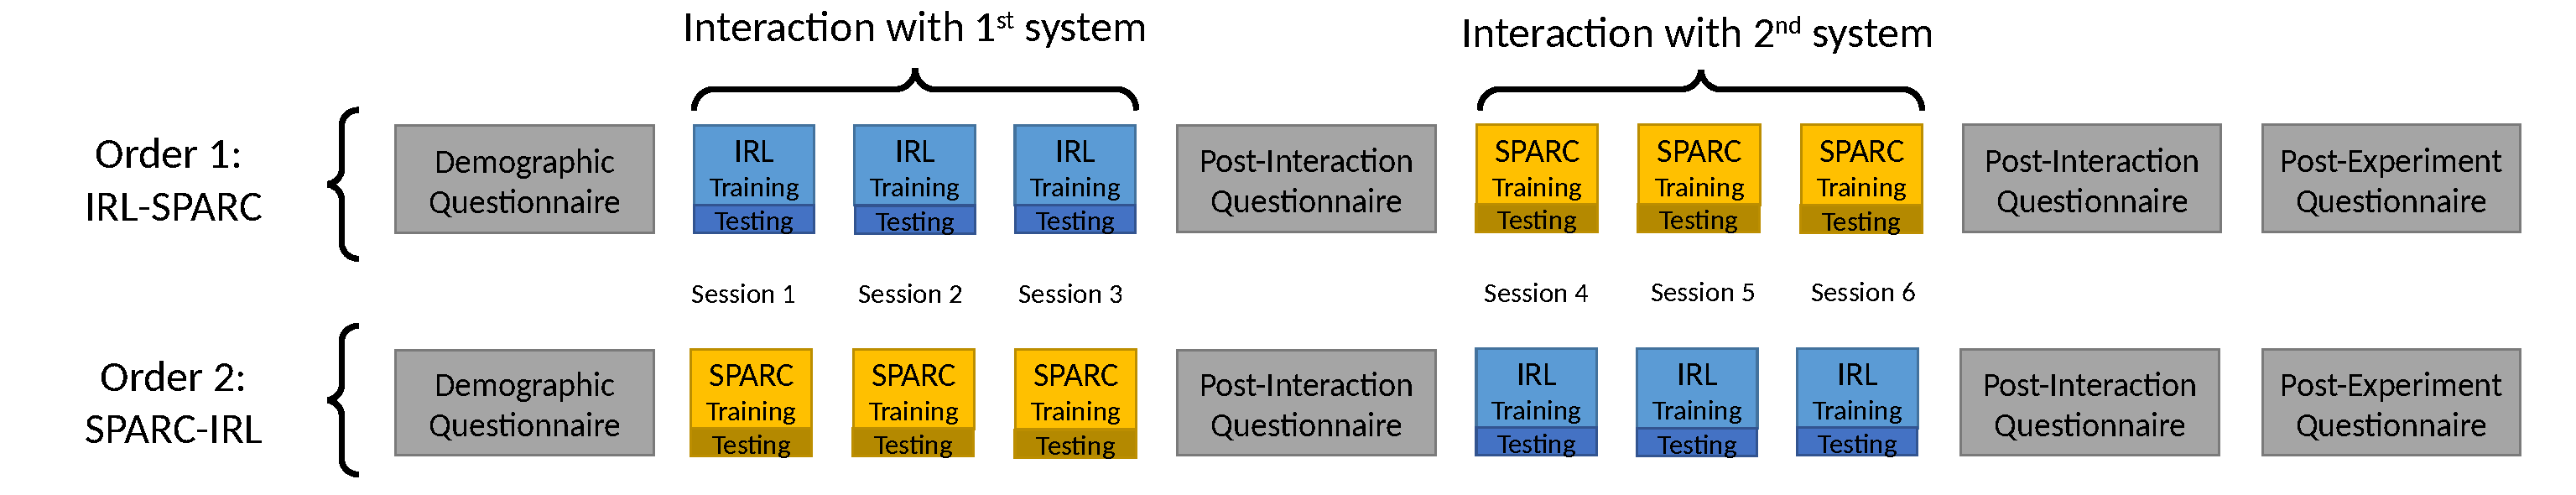
\includegraphics[width=1\textwidth]{fullDesign.pdf}
	\caption{Participants are divided into two groups. They first complete a demographic questionnaire, then interact for three independent sessions (with a teaching and a testing phase each) with a system (IRL or SPARC). After a first post-interaction questionnaire, participants interact for another three sessions with the other system before completing the second post-interaction questionnaire and a final post-experiment questionnaire.}
	\label{fig:control_design}
\end{figure}

\subsection{Participants}

A total of 40 participants have been recruited using a tool provided by the university to reach a mixed population of students and non-student members of the local community.  All participants gave written informed consent, and were told of the option to withdraw at any point. All participants received remuneration at the standard U.K. living wage rate, pro rata. Participants were distributed randomly between the groups whilst balancing gender and age (age \textit{M}=25.6, \textit{SD}=10.09; 24F/16M). Participants were mostly not knowledgeable in machine learning and robotics (average familiarity with machine learning \textit{M}=1.8, \textit{SD}=1.14; familiarity with social robots \textit{M}=1.45, \textit{SD}=0.75 - Likert scale ranging from 1 to 5).

In addition to naive non-expert users, an expert user (the author) interacted five times with each system following a strictly optimal strategy in both cases. These results from the expert are used to evaluate H2 and show the optimal characteristics of each system (\gls{irl} and \gls{sparc}) when used by trained experts such as therapist in a context of assistive robotics.

\subsection{Metrics}

\subsubsection{Interaction Metrics}

We collected four metrics during the teaching phase: the teaching performance (how many steps participants reached in the teaching phase), the teaching time (from 0 to 25 minutes), the number of times a participant reached a failure state while teaching (which can be related to the risks taken during the teaching) and the number of inputs provided during the teaching, which can be seen as the efforts invested in the teaching. The testing phase is a single run of the taught action policy ending as soon as the robot reaches an ending state (failure or success) or if stopped by the participants. We use the performance achieved during this single test as evaluation of the success of the teaching. As not all participants reached a success during the testing phase, we used the six key steps defined in Section \ref{ssec:control_task} as a way to evaluate the performance ranging from 0 (no step has been completed) to 6 (the task was successfully completed) during this testing run: for example a testing where the robot puts both ingredients in the bowl but reaches a failure state before mixing them would have a performance of 3.

\subsubsection{Questionnaires}

The post-interaction and post-experiment questionnaires provide additional subjective information to compare with the objective results from the interaction data. Two principal metrics are gathered: the workload on participants and the perception of the robot. 

Workload is an important factor when teaching robots. As roboticists, our task is to make the teaching of robots as undemanding as possible, meaning that the workload for user should be minimal. Multiple definitions for workload exist and various measures can be found in the literature. Due to its widespread use in human factors research and clear definition and evaluation criteria, we used the NASA-Task Load Index (TLX) \citep{hart1988development}. We averaged the values from the 6 scales (mental, physical and temporal demand, performance, effort and frustration) to obtain a single workload value per participant for each interaction. There are two measures for each participant, after the interaction with the first system and after the interaction using the other one.

Finally, the perception of the robot has been evaluated in the post-interaction and post-experiment questionnaires using subjective questions (measured on a Likert scale), binary questions (which robot did you prefer interacting with) and open questions on preference and naturalness of the interaction. 

\section{Results}

Most of the results are non-normally distributed. Both ceiling and floor effects can be observed depending on the conditions and the metrics. For the teaching time, some participants preferred to interact much longer than others, resulting in skewed data. Likewise for the performance: often participants either reached a successful end state or did not hit any of the sub-goals of the task in the testing phase ending often in two clusters of participants: one at a performance of 6 and one at 0.  Similarly, some participants who interacted a long time with the system did not complete any step, while others could achieve good results in a limited time. Due to the data being not normally distributed, Bayesian statistics have been used from the JASP software \citep{jasp2018}. Each test: mixed Anova for omnibus comparison between condition for each interaction (first or second), independent t-test for post-hoc comparison between participants and paired samples t-test for post-hoc comparison within participants have been performed using their Bayesian counterpart, which also remove the need of doing a correction on post-hoc test such as Bonferroni. As such, no p-value is reported, but a B factor representing how much a parameter impact of a parameter on the metric (if $B < 1/3$ there is no impact, if $B > 3$ the impact is strong) \citep{dienes2011bayesian,jeffreys1998theory}.

Initial results of the first interaction of the participants have been reported in \cite{senft2016providing}.

%\subsection{Interpreting results}

\subsection{Interaction data}

Five objective metrics (teaching performance, testing performance, teaching time, number of inputs provided and number of failures) and one subjective metric (workload) have been used to evaluate the efficiency of \gls{irl} and \gls{sparc}. 

\subsubsection{Teaching Performance}

Figure \ref{fig:control_teaching_performance} presents the performance of participants during the teaching phase, i.e how far in the steps they brought the robot during the teaching. It can be seen as how much control a method provide to the teacher and how easy it is to guide the robot to execute a desired action policy. It is also an upper bound for the testing performance as, due to the risk of failures or loop in the environment, the performance in the testing phase cannot (or has dramatically low probability to) achieve a higher performance than in the teaching phase.

In the first three sessions participants interacted with either \gls{irl} or \gls{sparc} and swapped for the remaining three sessions. The bayesian analysis shows the importance of the interacting condition on the teaching performance on the three sessions both for the first interaction and the second one ($B_1=2881$ and $B_2 = 76.2$). According to the medians and the graph, participants using \gls{sparc} achieved a higher teaching performance than the ones using \gls{irl}. The session number has no impact on the performance ($B_1=0.089$ and $B_2=0.105$). Table \ref{tab:control_teaching_perf} presents descriptive statistics of the performance in the different conditions.


\begin{figure}[ht]
	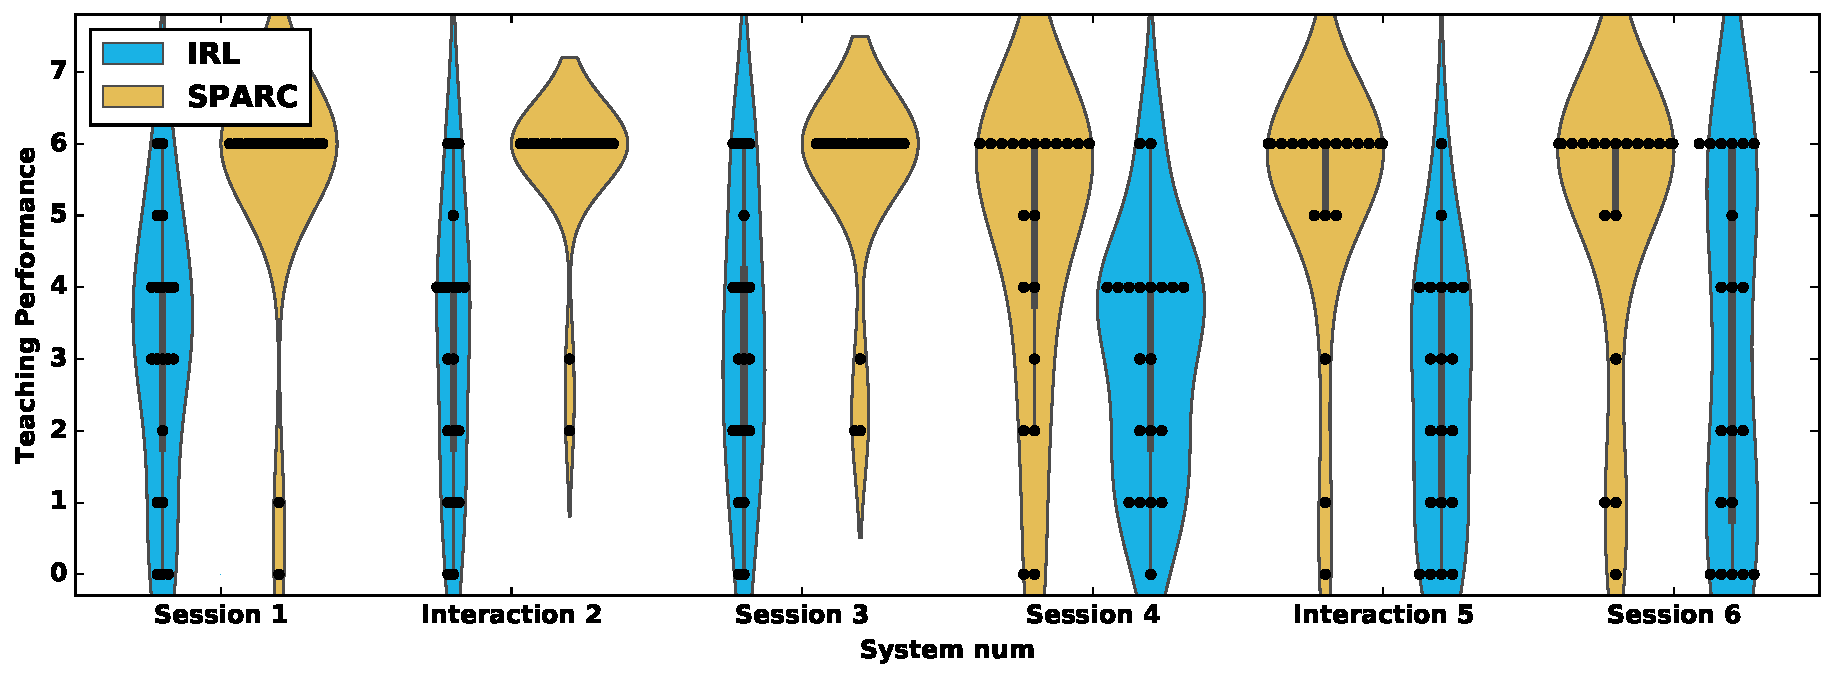
\includegraphics[width=\textwidth]{teaching_performance.pdf}
	\centering
	\caption{Comparison of the teaching performance for the six sessions (three with each system, IRL and SPARC, with interaction order balanced between groups). A 6 in teaching performance shows that the participant reached at least one success in the teaching phase.
	}
	\label{fig:control_teaching_performance}
\end{figure}

\begin{table}[ht]
	\centering
	\caption{Medians of the performance in the teaching phase. Lines represent the condition in which participant interacted in a the first three sessions or the last three. It must be noted that between session 3 and 4 participants change condition.}
	\label{tab:control_teaching_perf}
	\begin{tabular}{l"ccc|ccc}
		& $\widetilde{X}_{1}$ & $\widetilde{X}_{2}$ & $\widetilde{X}_{3}$ & $\widetilde{X}_{4}$ & $\widetilde{X}_{5}$ & $\widetilde{X}_{6}$\\ 
		\hline
		IRL & 3.0 & 3.5 & 3.0 & 3.5 & 2.5 & 3.0\\
		SPARC & 6.0 & 6.0 & 6.0 & 6.0 & 6.0 & 6.0\\
	\end{tabular}
\end{table}

\subsubsection{Testing Performance}

Figure \ref{fig:control_perf} presents the performance of participants during the testing phase, how successful was the teaching. The bayesian analysis shows important factor of condition on the performance on the three sessions both for the first interaction and the second one ($B_1=8.8$x$10^5$ and $B_2 = 7340$). The descriptive statistics show that participants using \gls{sparc} reached a higher performance than the ones using \gls{irl}. The session number has no impact on the performance on the first interaction, but results are inconclusive for the impact of repetition on the second interaction ($B_1=0.084$ and $B_2=0.80$). Table \ref{tab:control_perf} presents descriptive statistics of the performance in the different conditions.

 %There is a significant difference of performance between systems; a Friedman test shows a significant difference between systems during the first three sessions ($\chi^{2} = 50.8$, $p <.001$) and during the next three sessions ($\chi^{2} = 36$, $p <.001$). Similarly, a significant difference in performance is noted within participants (Order 1: $\chi^{2} = 37.9$, $p <.001$ - Order 2: $\chi^{2} = 55.3$, $p <.001$). 
 %In all the cases, participants interacting with \gls{sparc} achieved a significantly higher performance than those interacting with \gls{irl}, regardless of the order in which they interacted ($p<.05$ for all pairwise comparison). No difference of performance has been observed when using Wilcoxon signed rank test on the three repetitions between participants when interacting with the same system, so interacting for a second or third session with the same system does not have a significant impact on participants' performance.

As shown by table \ref{tab:control_perf}, in our study, only a limited number of participants succeeded in teaching the robot to complete the task using \gls{irl}, this observation will be discussed in more details in section \ref{sec:control_discussion}.


\begin{figure}[ht]
	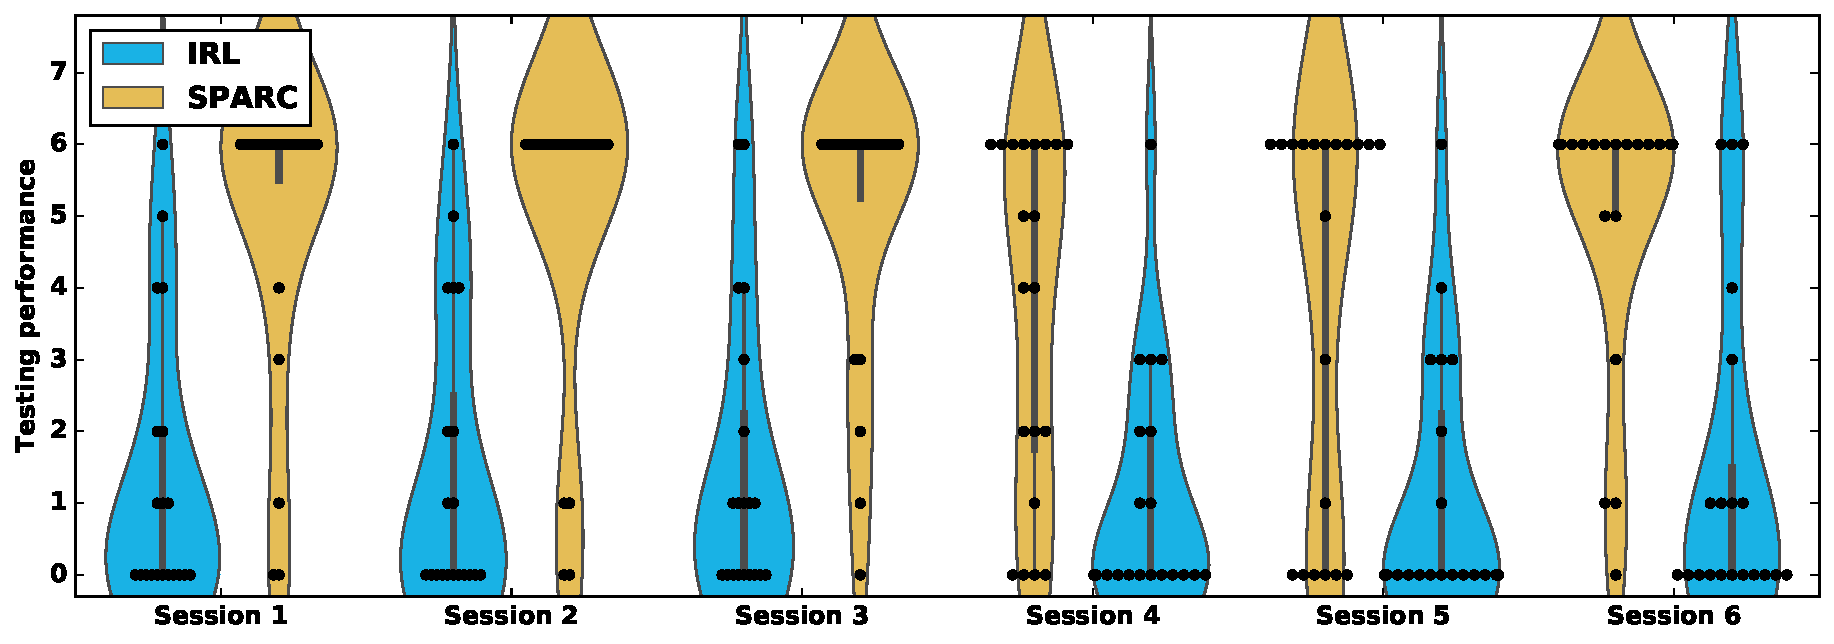
\includegraphics[width=\textwidth]{performance.pdf}
	\centering
	\caption{Comparison of the testing performance for the six sessions. A 6 in performance shows that the taught policy led to a success.
	}
	\label{fig:control_perf}
\end{figure}

\begin{table}[ht]
	\centering
	\caption{Medians of the performance in the testing phase.}
	\label{tab:control_perf}
	\begin{tabular}{l"ccc|ccc}
		& $\widetilde{X}_{1}$ & $\widetilde{X}_{2}$ & $\widetilde{X}_{3}$ & $\widetilde{X}_{4}$ & $\widetilde{X}_{5}$ & $\widetilde{X}_{6}$\\ 
		\hline
    IRL & 0.0 & 0.0 & 1.0 & 0.0 & 0.0 & 0.0\\
    SPARC & 6.0 & 6.0 & 6.0 & 4.5 & 6.0 & 6.0\\
	\end{tabular}
\end{table}

\subsubsection{Teaching time}

Figure \ref{fig:control_time} presents the time participants spent teaching. They could stop whenever they decided (if they think the robot masters the task or cannot learn further) or the  session would stop after 25 minutes. The bayesian analysis shows the important role of condition ($B_1=31.4$ and $B_2 = 679$) and sessions on the time spend teaching ($B_1=8.3$x$10^9$ and $B_2 = 3188$). Additional post-hoc comparisons for sessions indicate that in the first interaction, the teaching time decreases between the first and the second session and then tends to stabilise between the second and the third sessions ($B_{12}=4.4$x$10^5$, $B_{13}=2.6$x$10^6$ and $B_{23}=0.435$). Similar results happen in the second interaction ($B_{45}=850$, $B_{46}=382$ and $B_{56}=0.172$) with more strengths on the stabilisation of teaching time between session 5 and 6.

Table \ref{tab:control_time} presents descriptive statistics of the teaching time in the different conditions.

\begin{figure}[ht]
	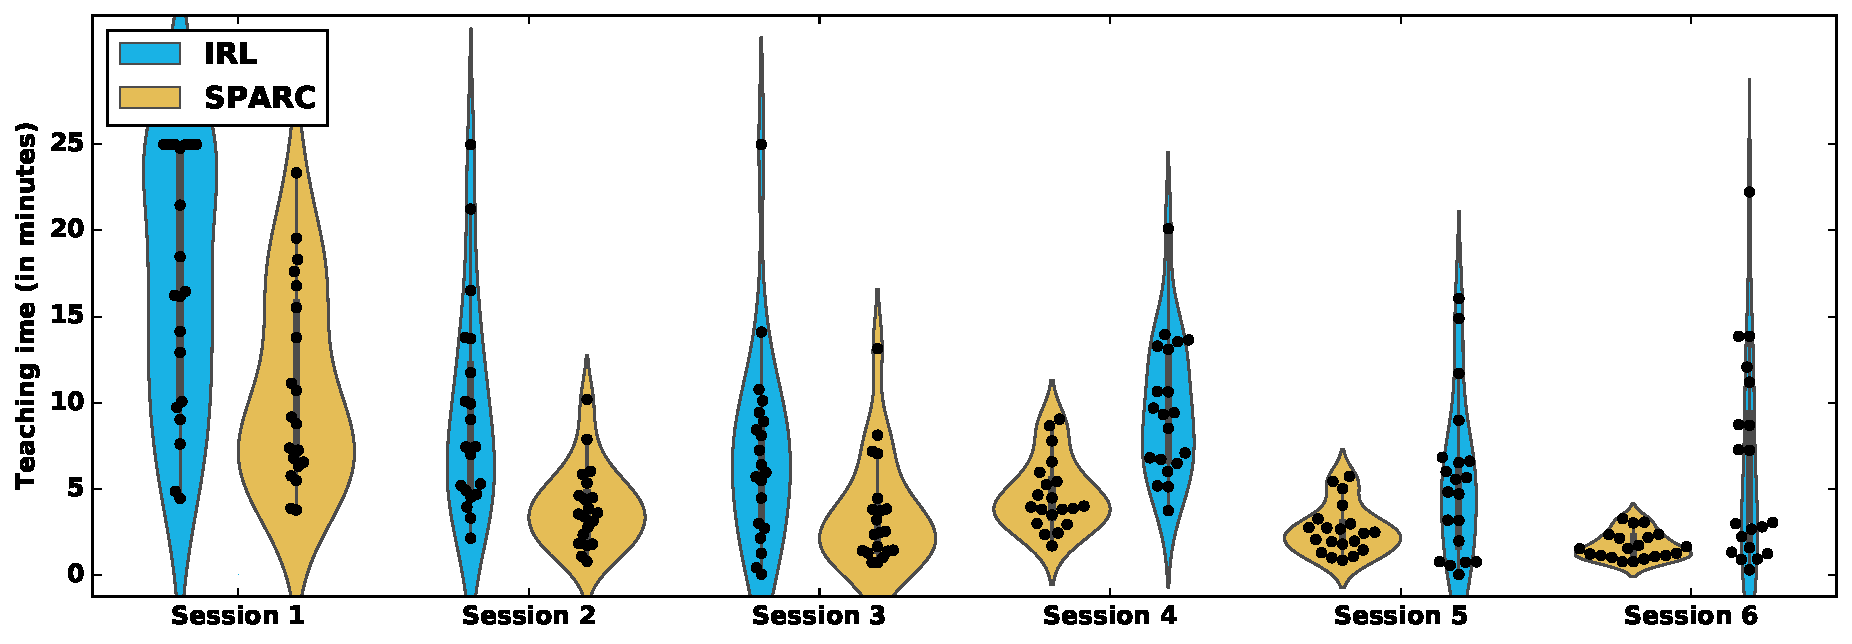
\includegraphics[width=\textwidth]{time.pdf}
	\centering
	\caption{Comparison of the teaching time for the six sessions. At 25 minutes, the session stopped regardless of the participant stage in the teaching.
	}
	\label{fig:control_time}
\end{figure}

\begin{table}[ht]
	\centering
	\caption{Medians of the teaching time in each session (in minutes).}
	\label{tab:control_time}
	\begin{tabular}{l"ccc|ccc}
		& $\widetilde{X}_{1}$ & $\widetilde{X}_{2}$ & $\widetilde{X}_{3}$ & $\widetilde{X}_{4}$ & $\widetilde{X}_{5}$ & $\widetilde{X}_{6}$\\ 
		\hline
    IRL & 16.34 & 7.43 & 6.16 & 9.36 & 5.18 & 3.0\\
    SPARC & 8.97 & 3.56 & 2.49 & 3.96 & 2.45 & 1.53\\
	\end{tabular}
\end{table}

\subsubsection{Inputs}
%To write
Figure \ref{fig:control_inputs} presents the number of inputs the participants provided while teaching. The bayesian analysis shows that in both interaction, the condition impacts the number of inputs provided ($B_1=27.4$ and $B_2 = 34.1$), while sessions matter highly in the first interaction, but the results are inconclusive for the second interaction ($B_1=4.1$x$10^5$ and $B_2 = 1.5$). Additional post-hoc comparisons for sessions indicate that in the first interaction, the number of inputs used decreases between the first and the second session and then tends to stabilise between the second and the third one($B_{12}=2707$, $B_{13}=4.7$x$10^4$ and $B_{23}=0.410$). However, for the second interaction, no strong difference is observed between session 1 and 2 and session 1 and 3 while the number of inputs stabilise between session 5 and 6 ($B_{45}=2.6$, $B_{46}=2.7$ and $B_{56}=0.17$).

Table \ref{tab:control_inputs} presents descriptive statistics of the number of inputs used in the different conditions.


\begin{figure}[ht]
	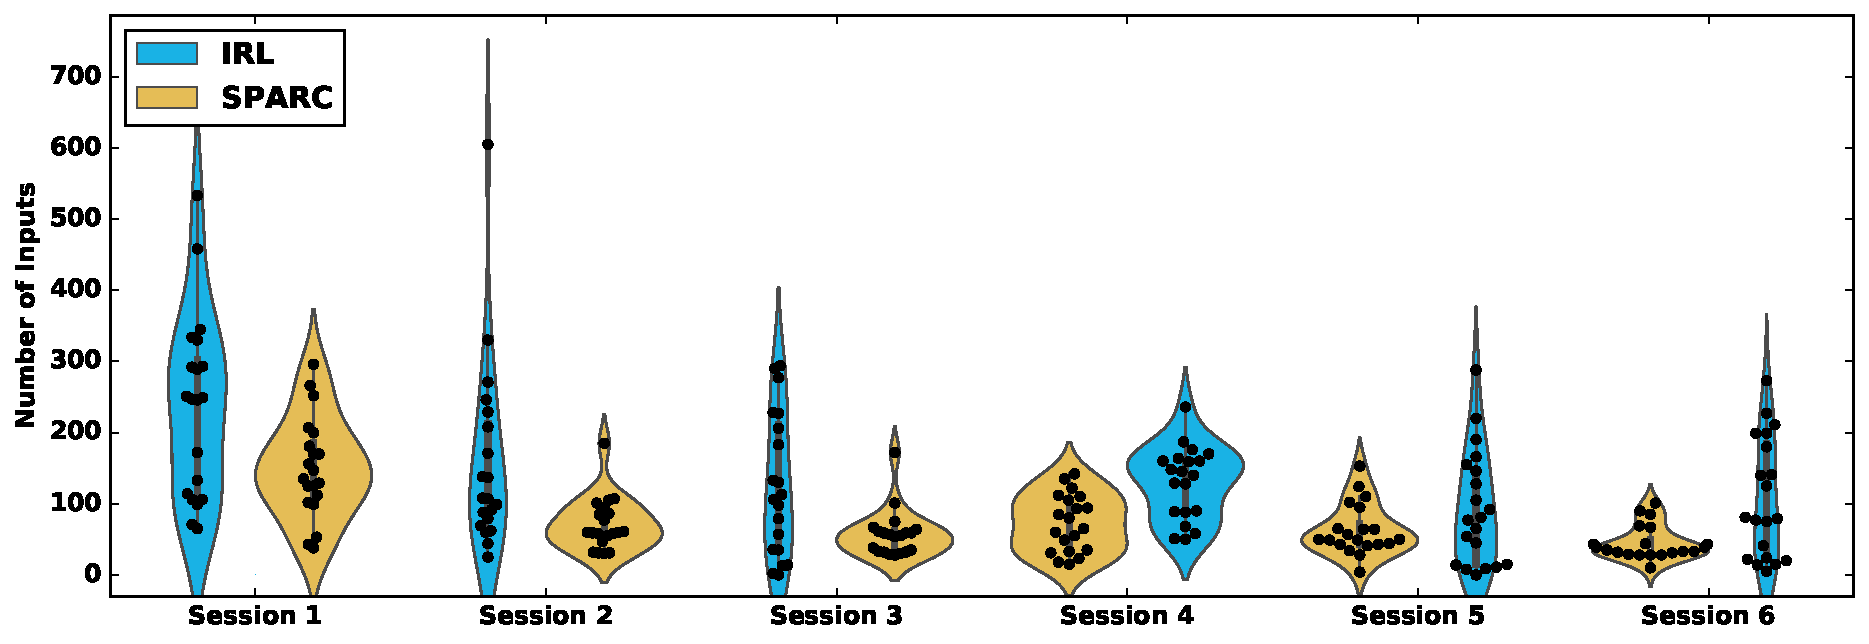
\includegraphics[width=\textwidth]{inputs.pdf}
	\centering
	\caption{Comparison of the number of inputs provided by the participants for the six sessions. 
	}
	\label{fig:control_inputs}
\end{figure}

\begin{table}[ht]
	\centering
	\caption{Medians of the number of inputs in the testing phase.}
	\label{tab:control_inputs}
	\begin{tabular}{l"ccc|ccc}
		& $\widetilde{X}_{1}$ & $\widetilde{X}_{2}$ & $\widetilde{X}_{3}$ & $\widetilde{X}_{4}$ & $\widetilde{X}_{5}$ & $\widetilde{X}_{6}$\\ 
		\hline
    IRL & 248.0 & 107.5 & 109.5 & 142.5 & 79.0 & 80.0\\
    SPARC & 141.0 & 60.0 & 56.0 & 72.5 & 50.0 & 37.0\\
	\end{tabular}
\end{table}

\subsubsection{Number of failures}

Figure \ref{fig:control_failures} presents the number of failures participants faced during the teaching phase. The bayesian analysis shows that for both interactions, both the condition ($B_1=6.2$x$10^4$ and $B_2 = 2.6$x$10^4$) and sessions ($B_1=1.5$x$10^4$ and $B_2 = 11$) have an important role on the number of failures. Additional post-hoc comparisons for sessions indicate that in the first interaction, the number of failures decreases between the first and the second session and then stabilises between the second and the third one($B_{12}=619$, $B_{13}=1.7$x$10^3$ and $B_{23}=0.25$). Similar results can be observed in the second interaction ($B_{45}=3.3$, $B_{46}=7.5$ and $B_{56}=0.2$).

Table \ref{tab:control_failures} presents descriptive statistics of the performance in the different conditions.

\begin{figure}[ht]
	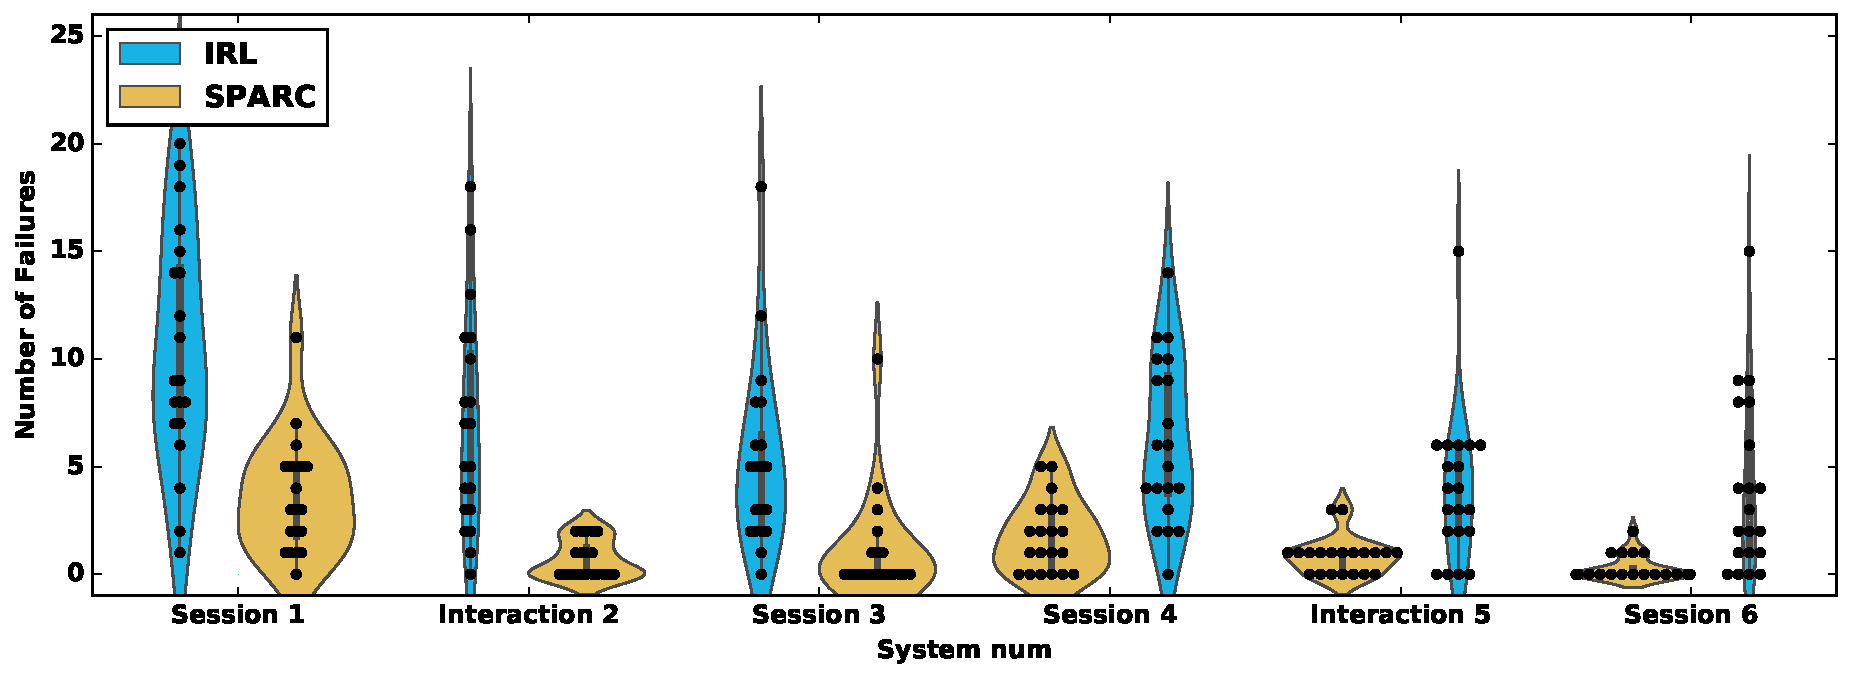
\includegraphics[width=\textwidth]{failures.pdf}
	\centering
	\caption{Comparison of the number of failures for the six sessions. A 6 in performance shows that the taught policy leads to a success.
	}
	\label{fig:control_failures}
\end{figure}

\begin{table}[ht]
	\centering
	\caption{Medians of the number of failures in the testing phase.}
	\label{tab:control_failures}
	\begin{tabular}{l"ccc|ccc}
		& $\widetilde{X}_{1}$ & $\widetilde{X}_{2}$ & $\widetilde{X}_{3}$ & $\widetilde{X}_{4}$ & $\widetilde{X}_{5}$ & $\widetilde{X}_{6}$\\ 
		\hline
	    IRL & 9.0 & 6.0 & 5.0 & 5.5 & 3.5 & 2.5\\
	    SPARC & 3.0 & 0.0 & 0.0 & 1.5 & 1.0 & 0.0\\
	\end{tabular}
\end{table}


\subsection{Questionnaire data}

The main task of the questionnaires was to assess the workload on participants when interacting with a condition. Figure \ref{fig:control_workload} presents the workload for participants for each condition for both interactions. Bayesian analysis show a strong effect on the condition for both interactions ($B_1=462$ and $B_2=8.1$x$10^4$) between participants and for both interactions order within participants($B_{SPARC-IRL}=1.1$x$10^4$ and $B_{IRL-SPARC}=1.7$x$10^6$). Regardless of the comparison criteria, when interacting with \gls{sparc}, participants reported a lower workload than when interacting with \gls{irl}. In the first interaction, participants using \gls{irl} reported a workload of 12.9 ($SD=2.33$), whereas the ones using \gls{sparc} reported 8.94 ($SD=3.01$). In the second interaction, participants interacting with \gls{sparc} rated their workload as 7.44 ($SD=3.41$) and the ones using \gls{irl} reported 13.87 ($SD=2.84$).

\begin{figure}[ht]
	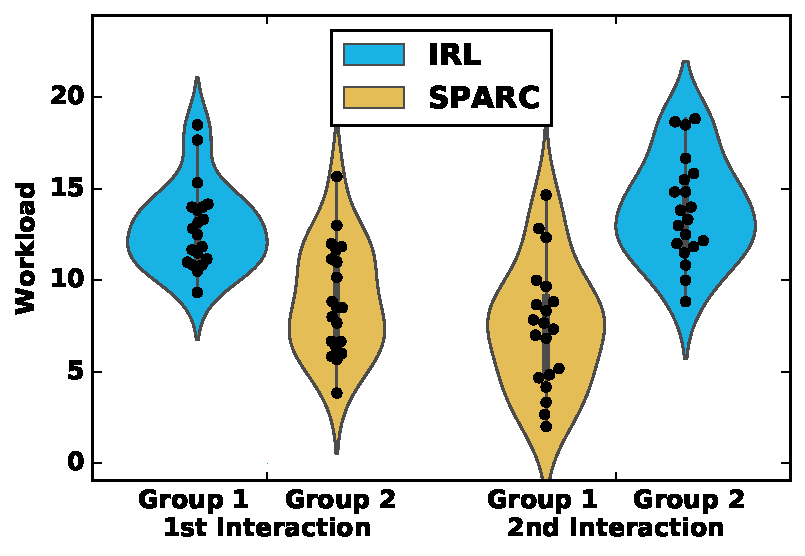
\includegraphics[width=.5\textwidth]{workload.pdf}
	\centering
	\caption{Workload as measured by the NASA-TLX for both conditions and both interaction order.
	}
	\label{fig:control_workload}
\end{figure}

\subsection{Expert} \label{ssec:control_expert}

To evaluate the best case potential offered by \gls{sparc} and \gls{irl}, an expert (the author) interacted five times with each systems. In both cases, the expert followed a strictly optimal strategy. This shows the expected behaviours in optimal conditions, the best metrics achievable. Results of the interactions are presented in Table \ref{tab:control_expert}. In both cases, the expert successfully taught the robot (as indicated by a performance of 6), which indicates that both systems can be used to teach a robot an action policy. However the time required to teach the robot with \gls{irl} is higher than with \gls{sparc} ($B=7102$). 

Additionally, when using \gls{irl}, even an expert cannot prevent the robot from reaching failure states during the teaching due to the lack of control over the robot's action. This is prevented when interacting with \gls{sparc}, due to the full control and clear communication, the teacher can ensure that only desired actions are executed. So with sufficient knowledge, an expert can teach the robot to behave safely without having to explore and reach undesired states. This has real world applications, as random exploration is often impossible or undesirable, \gls{sparc} offers a way for the teacher to stop the robot from executing actions with negative consequences.

Similar results have been observed with the non-expert participants: in their last interaction with \gls{sparc}, both groups had a median of 0 failures for a performance of 6, meaning that more than half of the participants successfully taught the robot the task without ever hitting a failure state after understanding how \gls{sparc} can be used.

\begin{table}[ht]
	\centering
	\caption{Results of an expert interacting 5 times with each system following an optimal strategy. In case without variance, Bayes Factor cannot be computed.}
	\label{tab:control_expert}
	\begin{tabular}{cccc}
	&IRL \textit{M(SD)} & SPARC \textit{M(SD)} & $B$ factor\\
		\midrule
		Performance & 6 (0) & 6 (0) & NA \\
		Time (minutes) & 4.5 (0.67) & 0.60 (0.03) & 7102 \\
		Inputs & 115.6 (8.4) & 28 (0) & NA \\
		Number of Failures & 3.2 (0.84) & 0 (0) & NA \\
%		\bottomrule
	\end{tabular}
\end{table}

%\section{Discussion}

\section{Validation of the hypotheses}

\subsection{Effectiveness and efficiency with non-experts}
The objective data (teaching and testing performance, teaching time, number of inputs and number of failures) show that despite spending a shorter time interacting with \gls{sparc} and using less inputs, participants reached a higher performance than with \gls{irl} whilst facing fewer failures during the teaching. Additionally, when interacting with \gls{sparc}, participants' time required to teach the robot decreased with successive sessions, without affecting the performance. This indicates that after the first session, participants understood the interaction mechanism \gls{sparc} and consistently managed to achieve a high performance whilst requiring less time to teach the robot the task. On the other hand, when interacting with \gls{irl}, participants' performance remains low over the session, and their teaching time decreases between session 1 and 2 but not between session 2 and 3. This might be due to a loss of motivation after session 1 where often participants did not succeed to teach the robot, reducing the desire to further interact in successive sessions. 

The results suggest that teaching the robot using \gls{sparc} allows the robot to achieve a higher performance than with \gls{irl}, in a shorter time, while requiring fewer inputs and making fewer errors when teaching. These objective results are also supported by subjective measures: the workload on the teacher is lower when using \gls{sparc} than when using \gls{irl}. For these reasons, H1 ( `Compared to \gls{irl}, \gls{sparc} can lead to higher performance, whilst being faster, requiring fewer inputs and less mental effort from the teacher and minimising the number of errors during the teaching when used by non-experts.') is supported.

\subsection{Safety with experts}

As presented in Section \ref{ssec:control_expert}, when interacting with \gls{sparc}, experts can reach a success easily and safely (low number of inputs, quickly and without facing failures), and this effect is also observed after some training for the naive participants: most of them reached a success without encountering any failures in their last interaction with \gls{sparc}.

However, when interacting with \gls{irl}, even experts cannot prevent the robot to end in failures states even when applying a strictly optimal action policy. This effect is typical of feedback-based \gls{iml} methods: as the teacher only rates the actions of the agent, they cannot prevent them to make errors, they can just reward negatively these errors.

This shows support for H2 (`\gls{sparc} can be used by experts to teach an action policy safely, quickly and efficiently, unlike other \gls{iml} methods lacking control'). This also demonstrates how the principles presented in Chapter \ref{chap:sparc} can provide control to the teacher over the robot's actions and so improve the teaching and ensure that even in the early stages of teaching, the action policy of the robot can be appropriate, which is not the case of most other \gls{iml} methods.

%COntinue from here

\subsection{Control}
\label{sec:control}

One of the main differences between the two methods is the way in which the concept of teaching is approached. With \gls{irl} an exploratory individual learning approach is followed: the robot has freedom to explore, and it can receive feedback on its actions and hints about actions to pursue next from a teacher. This is to some extent inspired by how children are taught, where the learning process can be more important than the achieved results. This is supported by the behaviours observed by Thomaz and Breazeal: their participants gave motivational rewards to the robot, just as one would to do to keep children motivated during learning, despite the absence of effect or use in classical reinforcement learning.

On the other hand, \gls{sparc} promotes a more direct teaching process: the supervisor explicitly tells the robot what to do and expects it to obey and learn. The robot is not totally considered as a social agent from the supervisor's point of view, but rather as a tool having to learn an action policy. This does not mean that the robot cannot be social: the supervisor can teach in such a non-social way to the robot how to interact socially. This approach is more task oriented, and we argue that it better fits assistive robotics when the interaction with the teacher does not have to be social, and the task (such as interaction with a child with \gls{asd}) is more important than the social relation between the robot and its supervisor (a therapist for example).

The post-experiment questionnaire included the open question: `which robot did you prefer interacting with and why?'. Almost all the participants (38 out of 40) replied that they preferred interacting with \gls{sparc}. Half of all the participants used vocabulary related to the control over the robot actions (`control', `instruction', `command', `what to do' or `what I want') to justify their preferences without these words being used in the question. Furthermore, multiple participants reported being frustrated to have only partial control over the robot's actions with \gls{irl}, they would have preferred being able to control each action of the robot. 

To the question `which interaction was more natural?', 10 participants rated \gls{irl} as being more natural, using justifications such as: `The robots thinks for itself', `Some confusion in the [\gls{irl}] robot was obvious making it more natural', `More like real learning', `Because it was hard to control the robot' or `People learn from their mistakes faster'. But despite acknowledging that \gls{irl} is more natural, closer to human teaching, participants still preferred teaching using \gls{sparc}. This suggests that when humans teach robots, they are focused on the results of the teaching: can the robot do the new task requested. This relates to the role of robots, they often interact in human-centred scenario where they have to complete a task for their users. And due to the absence of life-long learning for robots today, it is not worth investing time and energy to allow the robot to improve its learning process or explore on its own. These comments from the participants show support for H3 (`Teachers prefer a method providing more control over the robot's actions.').

\section{Discussion}
\label{sec:control_discussion}

Despite not being originally designed to be used in combination with \acrlong{rl}, \gls{sparc} does achieve good results. This shows that principles presented in Chapter \ref{chap:sparc} are agnostic to the learning algorithm and promote efficient teaching. Furthermore, \gls{sparc} achieves a higher performance, in a shorter time and facing less failures than \gls{irl}, whilst requiring a lower workload from the human teacher. And finally, when used by experts, \gls{sparc} demonstrates that teaching can be safe and quick: the full control over robot's action in the teacher's hands ensures that only desired actions will be executed. These results show an important feature of teaching; as robots interact in task oriented, human-centred environments, human teachers seem to prefer direct approaches focused on commands rather than letting the robot explore on its own.

\subsection{Comparison with original Interactive Reinforcement Learning study}

Unlike in the original experiments evaluating \gls{irl} \citep{thomaz2008teachable}, in this study, most of the participants did not succeed in teaching the robot the full cake baking sequence using feedback and guidance. In the \citet{thomaz2008teachable} study, the participants were knowledgeable in machine learning (M=3.7, SD=2.3 - range: 1 to 7), but the population in the current study was drawn from a more general public having little to no knowledge of machine learning (M=1.8, SD=1.13 - range: 1 to 5). This can explain why a much larger number of participants did not achieve success with \gls{irl} in this study whereas Thomaz and Breazeal only reported 1 participant out of 13 failing the task. In our study, 12.5\% of the participants and the expert did manage to teach the robot using \gls{irl}. As demonstrated by the teaching performance, most of the participants did not manage to reach a single success during the teaching phase. We identify the lack on control over the robot's actions as limiting factor for the teaching, as participants did not manage to steer the robot to do correct actions, they could not reward it and teach it an action policy. Additionally, the requirement of explicit feedback made the learning task more complex. Future robot teachers need to have control over the robot's action if they have to teach them action policies and robots should also use implicit rewarding to ease the task for the teacher. 
%This seems to be largely due to participants not consistently rewarding correct actions, preventing the reinforcement learning algorithm from learning. This is why implicit rewards --every action allowed by the teacher is positively rewarded-- tend to work better than explicit ones. 
This is consistent with \cite{kaochar2011towards} who note that feedback is not well suited for teaching an action policy from scratch, but better for fine tuning. For teaching the basis of the action policy, they recommend using demonstrations, a method much closer to \gls{sparc}. 

\subsection{Advantages and limitations of SPARC}

In the \gls{sparc} implementation for this study, \gls{sparc} reproduces actions selected by the teacher. So one can argue that no learning algorithm is required, instead the actions could just be blindly reproduced by the robot. However, when combined with reinforcement learning, \gls{sparc} does provide advantages: due to the Q-Table, all the loops in the demonstration are removed when the robot interacts on its own and it provides a way to deal with variations in teaching. It also allows the robot to continue from any state in the trajectory. And finally, due to the suggestion/correction mechanism, the teacher can leave the robot to act on its own as long as it attempts correct actions, and the human to intervene only when the robot is about to execute an incorrect action. 

%PRobably not required
%Over the 79 successful trials using \gls{sparc}, participants used 47 different strategies to teach the robot the task of baking a cake. This shows how \gls{sparc}, as a single control mechanism, allows for different action policies to be learnt depending on the person teaching the robot. With \gls{sparc} the robot can adapt its behaviour to the human it is interacting with, profiling the user to find the desired way of behaving.

However \gls{sparc} also has limitations in the current implementation, related to the quality of the human supervised guidance. If the teacher allows an action to be executed by mistake (through inattention or by not responding in time), this action will be reinforced and will have to be corrected later on. This might lead to loops when successive actions are cancelling each other (such as move left, then right). In that case, the teacher has to step in and manually guide the robot to break this cycle. Furthermore, due to the automatic execution of actions, the teacher has to be attentive at all times and ready to step in when a wrong action is suggested by the robot.

In this version, \gls{sparc} has been applied to a scenario where a clear strategy with optimal actions is present. The interaction also takes place in a virtual environment with a discrete time. Real human-robot interactions are stochastic, happen in real time and often there is no clear strategy known in advance. However, we argue that human experts in the application domain can know what type of actions should be executed when, and which features of the environment they used for their decision. As this knowledge can not be available to the robot's designers, robots should be able to learn from a domain user in an interactive fashion. In the chapter, \gls{sparc} mainly receives inputs from a teacher at predefined discrete times and still does not use the human knowledge to it's fullest: the learning algorithm is still simple and with limited inputs, but as presented in Chapter \ref{chap:education},  \gls{sparc} has been tested in real-world interactions with humans.

%PRobably not required
%Nevertheless, we argue that \gls{sparc} allows for easy and safe teaching due to the presence and control by the teacher. And the suggestion/correction mechanism with automatic execution of actions allows for a smooth teaching process where the workload on the teacher can decrease over time as shown in \cite{senft2015sparc}. The workload of the teacher when starting is relatively high, when the robot has no information on which actions to take yet, and decreases over time requiring only limited intervention by the teacher.

%MIght be put in the final discussion
\subsection{Lessons learned on designing interactive machine learning for human-robot interactions}

From observing the participants interacting with both systems, we derived four recommendations for future designs of interactive learning robot that we also used to develop the study presented in Chapter \ref{chap:education}. 

\subsubsection{Clarity of the interface}

Algorithms used in machine learning often need precisely specified inputs and outputs and require an internal representation of the world and policies. These variables are often not accessible to a non expert: the weights of a neural network or the values in a Q-table are not easily interpreted, if at all. The inner workings of the machine learning algorithms are opaque, and people only have access to input and output of the black box that is machine learning. As such, care needs to go into making the input and output intuitive and readable. For example, in this study (following Thomaz and Breazeal's original study), the communication between the robot and the teacher occurred through the environment: using clicks on objects rather than buttons on a graphical user interface. This design decision has important consequences as participants first have to familiarise themselves with the interface: how to interpret the robot's behaviour, what actions are available for each state and what is the exact impact of the actions? This lack of clarity leads to a high number of failures and high teaching time during the first session in our study. So we argue that to avoid this precarious discovery phase for the teachers, roboticists have to design interfaces taking into account results from the Human Factors community as advocated by \cite{adams2002critical}.

\subsubsection{Limits of human adaptability}

Human-Robot Interaction today is facilitated by relying on people adapting to the interaction, often making use of anthropomorphisation \citep{zlotowski2015anthropomorphism}. Roboticists use people's imagination and creativity to fill the gaps in the robot's behaviour. However, human adaptivity has its limits: in our study, often participants adopted one particular way of interacting with the system and they hold on to it for a large part of the interaction. For example, participants clicked on an object requiring two actions to interact with, assuming that the robot had planning capabilities which it did not. Or when the robot was blocked in some cycles (due to constant negative reward in \gls{irl} or due to a loop created and not stopped with \gls{sparc}), participants kept on trying the same action to break the loop, without really exploring alternatives. For these reasons, if robots are to be used with a naive operator, they need a mechanism to detect these `incorrect' uses and either adapt to these suboptimal human inputs or they need to inform the user that this type of input is not supported and clarify what human behaviour is appropriate instead.

\subsubsection{Importance of keeping the human in the learning loop}

As argued in previous chapters, we think the presence of a human in the learning loop is key. This human in the loop can provide importance knowledge about the environment and allow the machine learning to deal with sensor errors or imperfect action policies. An expert supervising the robot should also be able to prevent the execution of specific actions or force the execution of others. This was one of the important points we considered when proposing \gls{sparc}: there is no distinction between a teaching and a testing phase, they are merged into a single phase. The teacher can correct the robot when needed and let it act when it behaves correctly. Participants used this feature of \gls{sparc} in this study: many participants corrected \gls{sparc} only when required rather than forcing every action, 37.5\% of the participants even let the robot complete the task without giving a single command before starting the test to be sure that the robot is ready. So \gls{sparc} has been used as a tool to provide online learning to a robot whilst keeping the teacher in control, but reducing the need of intervention over time in this study.

\subsubsection{Keeping people in control}

Most of the scenario where a robot has to learn how to interact with humans are human-centred: the robot has to complete a task to help a human (such as in socially assistive robotics). In these scenarios, the goal of the learning is to ensure that the robot can complete the task assigned to it, not to provide the robot with tools to learn more efficiently in further interactions. Similarly, participants in our study did not desire to have the robot exploring on its own and learn from its experience, they wanted to be able to direct the robot. Furthermore, a lack of control over the robot's actions can lead to frustration and loss of motivation for the teacher. This human control is especially critical when the robot is designed to interact with other people as undesired actions can have a dramatic impact, such as causing harm for the interaction partners or bystanders. For these reasons, we argue that when designing an interactively learning robot for Human-Robot Interaction in human-centred scenario, it is critical to keep the human in control. 

However, this control does not mean that the robot cannot learn and become autonomous. We take a stronger inspiration from \gls{lfd}, using human input more efficiently to guide the learning, speeding it up and making it safer, especially in the early stages of the learning. The human is in control mainly when the robot is prone to make exploratory mistakes, and can prevent them before they occur, but once the action policy is appropriate enough, the teacher can leave the robot learn mostly on its own and refine its action policy with limited supervision from a human.

%\subsection{Future work}
%\label{ssec:future}
%We are currently working on a new experiment in which people interacting with a robot in a continuous time and non-deterministic environment. In this experiment, the teacher is able to send commands to the robot, provide rewards and identify features in the environment they consider important. The learning algorithm will take these inputs into account and combine them with interaction metrics to learn. An approach could be to use the actor-critic paradigm: the critic being an objective evaluation of the action results (environmental rewards), and the actor using results from the critic and teacher's guidance to update the action policy.

\section{Summary}

As presented in Chapter \ref{chap:sparc}, \gls{sparc} has bee designed to allow naive human to teach an action policy to a robot while maintaining a constant appropriate behaviour. This chapter presents a study where \gls{sparc} was combined with \gls{rl} to teach a simulated robot to complete a baking task. \gls{sparc} used communication of intentions from the robot, full control of the teacher over the robot behaviour and implicit rewarding mechanism to have participants teach the robot an action policy. This approach has been compared with \gls{irl} using communication of uncertainty, partial control and explicit rewarding to teach the robot. When interacting with \gls{sparc}, participants reached more success, with less time and inputs and while facing fewer failures and a lighter workload than when interacting with \gls{irl}. From this user study involving 40 participants, \gls{sparc} has demonstrated being usable by naive participants to successfully teach an action policy and succeeded in its goal to enable humans to quickly and safely teach a robot an action policy.

Based on these results and other observations, we also propose four guidelines to design interactive learning robots: (1) the interface to control the robot has to be intuitive, (2) the limits of human adaptability have to be taken into account (robots should detect deadlocks in human behaviours and adapt their way to be controlled or inform the human about it), (3) the operator should be kept in the learning loop and (4) teachers should stay in control of the robot behaviour when interacting in sensitive environment. The first two points can be seen to apply to all robot teaching methods, and should be addressed at the time of designing the interface. And by definition, \gls{sparc} aims to address these last two points: maintaining the performance of an adaptive system by remaining under progressively decreasing supervision. 


